\section{Simulated Annealing Grasping}
\label{sec:sim_ann}

The \ac{SANN} algorithm~\cite{Ciocarlie2009} integrated in the ``GraspIt!'' simulator~\cite{AndrewT2004} is one of the tools that the grasping pipeline relies on. Since it was used from the perspective of an end user, a brief explanation will be done here. Further information can be retrieved on the referenced papers.

The \ac{SANN} is a heuristic optimization algorithm based on the cooling of a set of atoms to a minimum state of energy and it was first introduced by~\cite{kirkpatrick1983} in a Statistical Mechanics optimisation algorithm application. The ``Very Fast Simulated Re-Annealing'' was an improvement made by Ingber at~\cite{ingber1988} and used here. Since it is based on temperature, Ingber proposed that its cooling process decrease as described by Equation~\ref{eq:temperature}

\begin{equation}
T=T_{0} \cdot exp{(-k^{1/D})}
\label{eq:temperature}
\end{equation}

\noindent
where $D$ is the dimensional search space, $k$ a \ac{SANN} parameter step, and $T_0$ is the initial temperature.

Each algorithm iteration generates new state variables following a rule of neighbouring. Considering current and a new variable state as $S_{current}$ and $S_{new}$, this rule yields Equation~\ref{eq:neighbors}.

\begin{equation}
S_{new}=S_{current}+T \cdot(-1)^{round(Rand(0,1))} \cdot\left(1+\frac{1}{T}\right)^{Rand(-1,1)}
\label{eq:neighbors}
\end{equation}

\noindent
and the probability to change the state between the current and the new one is defined by Equation~\ref{eq:very_fast_snn_prob} where $Q(\bullet)$ represents the objective function of the optimization problem.

\begin{equation}
exp({\frac{Q(S_{current})-Q(S_{new})}{T}})>Rand(0,1)
\label{eq:very_fast_snn_prob}
\end{equation}

Regarding the multi-fingered grasping, it is possible to define a state based on the hand posture $\mathbf{p}$ and, the position and orientation of the wrist $\mathbf{w}$ such as:

%\begin{equation}
%S=[\mathbf{p}, \mathbf{w}], \quad \mathbf{p} \in \mathcal{R}^{d}, \mathbf{w} \in \mathcal{R}^{6}
%\label{eq:fob_grasp}
%\end{equation}

\begin{equation}
	\mathbf{S}=\left[\begin{array}{c}
		\mathbf{p} \\
		\mathbf{w}\end{array}\right], \quad \mathbf{p} \in \mathcal{R}^{d}, \mathbf{w} \in \mathcal{R}^{6}
\label{eq:fob_grasp}
\end{equation}

\noindent
where $d$ is the number of intrinsic \acp{DOF} of the hand. For instance, the human hand and the robotic Barrett gripper~\cite{barret_hand} have 20 \acp{DOF} and 4 \acp{DOF}, respectively.

As discussed by~\cite{Ciocarlie2009}, the hand posture is defined by \textit{eigengrasps}, a subspace of movement based on how human generate hand postures. The \textit{eigengrasps} reduces the \acp{DOF} of the hand based on how humans select appropriate grasps and hand postures in a primitive fashion. Studies show that humans simplify, unconsciously, the problem with a pattern in the movement. More information can be verified in~\cite{Ciocarlie2009,Santello2002}. 

Considering a hand with $d$ hand's postures DOFs, it is possible to defined a d-dimensional \textit{eigengrasp} ($\mathbf{e}_i$) as:

\begin{equation}
	\mathbf{e}_{i}=\left[\begin{array}{llll}
		e_{i, 1} & e_{i, 2} & \ldots & e_{i, d}
	\end{array}\right]
\end{equation}

\noindent where each $e_{i,d}$ represents the individual joint direction movement. In other words, the \textit{eigengrasp} ($\mathbf{e}_i$) is a d-dimensional direction vector that represents the motion of a group joint space. Therefore, it is possible to create a set of \textit{eigengrasps} with size $b \ll  d$, simplifying the searching space. Hence, a posture can be defined by Equation~\ref{eq:eigengrasp_posture}.

\begin{equation}
p=\mathbf{p}_m+\sum_{i=1}^{b} a_{i} \mathbf{e}_i
\label{eq:eigengrasp_posture}
\end{equation}


\noindent
with posture origin defined by $\mathbf{p}_m$ and $b$ the total number of \textit{eigengrasps}. Since it is a linear combination, the parameter array $\mathbf{a} = [a_1, a_2, ... , a_b]$  will be the optimisation variable in Equation~\ref{eq:fob_grasp} together with the $\mathbf{w}$. Therefore, the dimensional search space $D$ has a reduced length, i.e. $D = sizeof(\mathbf{a}) +  sizeof(\mathbf{w})$. The Figure~\ref{fig:barrett_eigengrasps} elucidates the \textit{eigengrasp} discussion in the case of 4 \ac{DOF} Barrett gripper.


\begin{figure}[h!]
	\resizebox{0.85\textwidth}{!}{%
		\begin{tcolorbox}
			\centering
			\begin{subfigure}[c]{.475\textwidth}
				\centering
				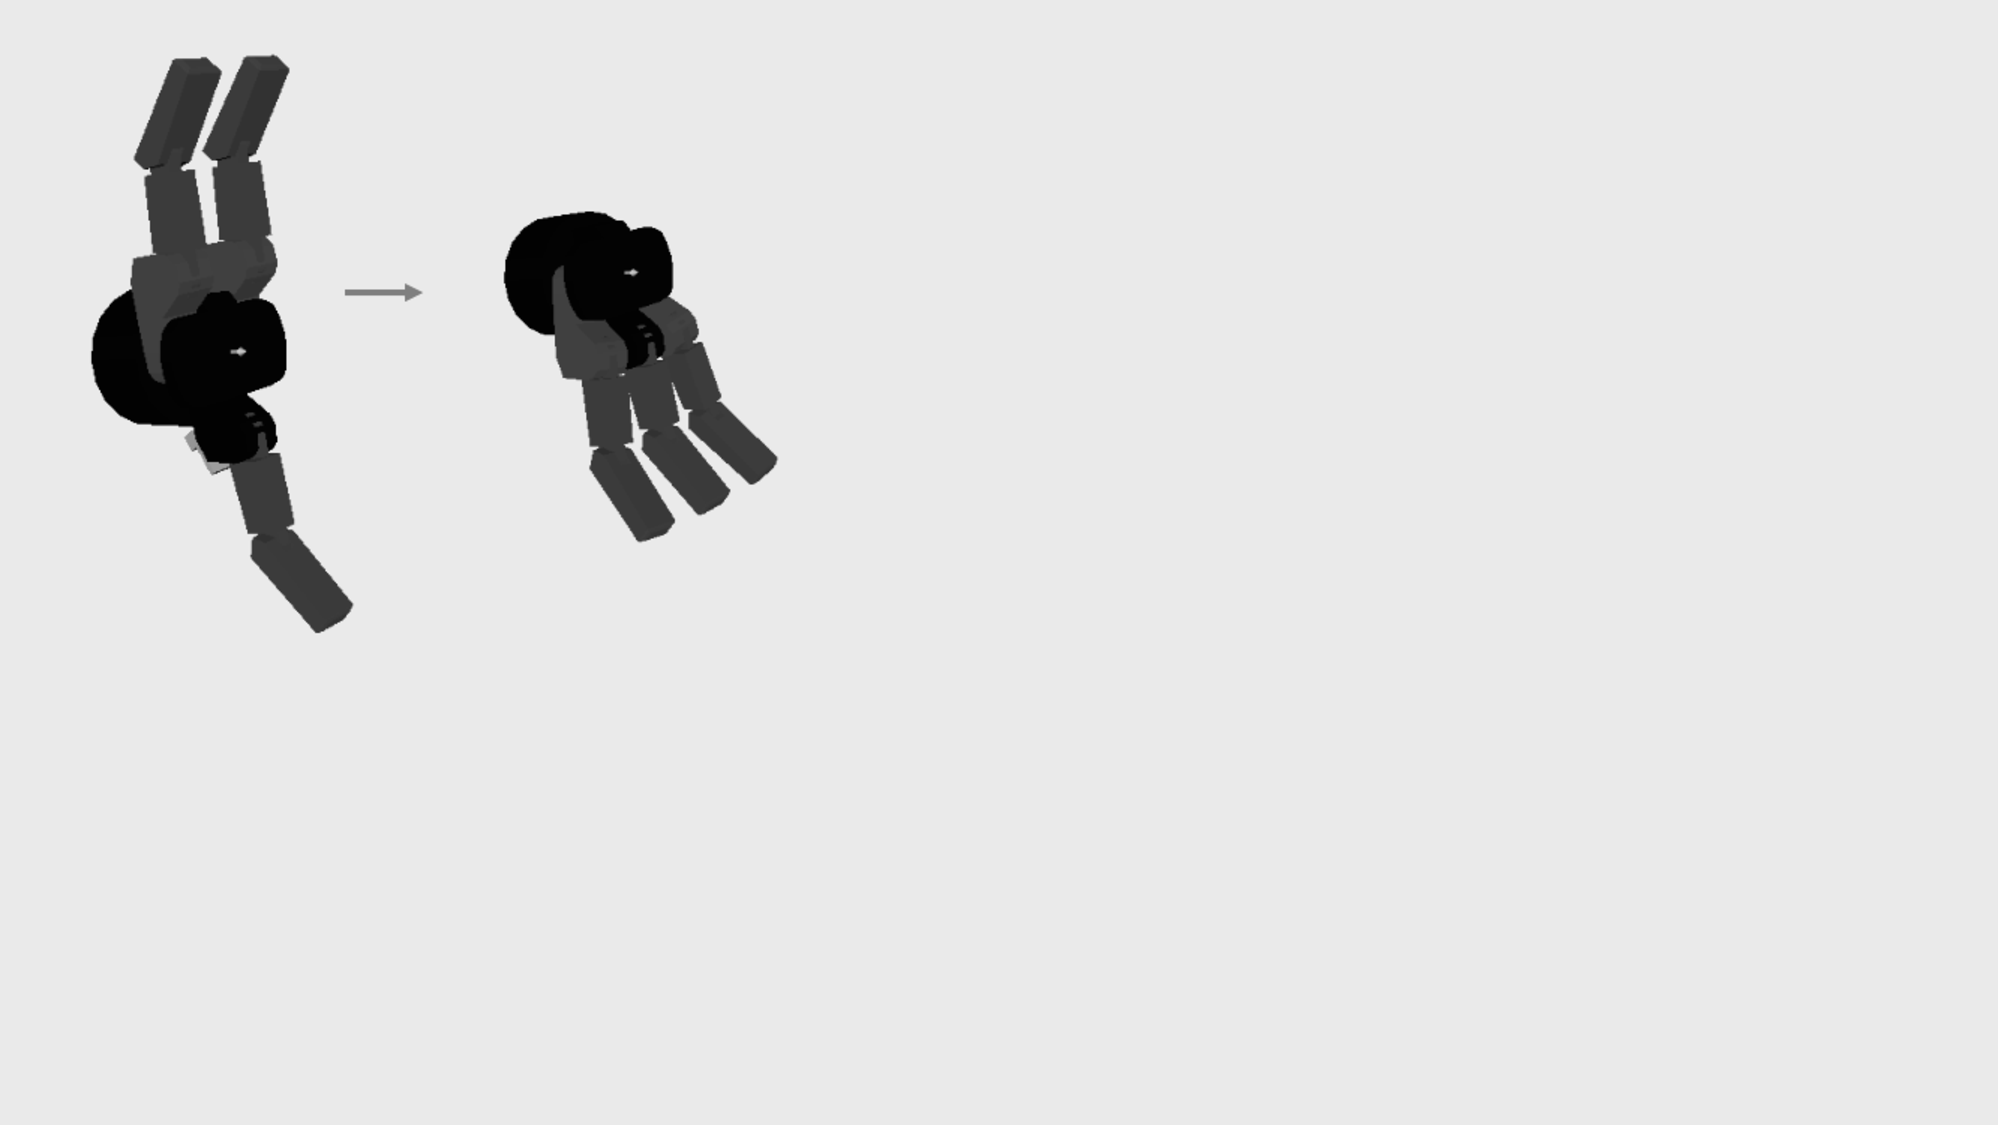
\includegraphics[trim={1cm 8cm 19cm 0cm},clip,width=1\linewidth,angle=0]{Apendices/Figuras/barret_eigengrasp_01.pdf}
				\caption{\textit{Eigengrasp} 01: fingers twist movement over wrist's normal axis.}
				\label{fig:barrett_eigengrasp01}
			\end{subfigure}
			\quad
			\begin{subfigure}[c]{.475\textwidth}
				\centering
				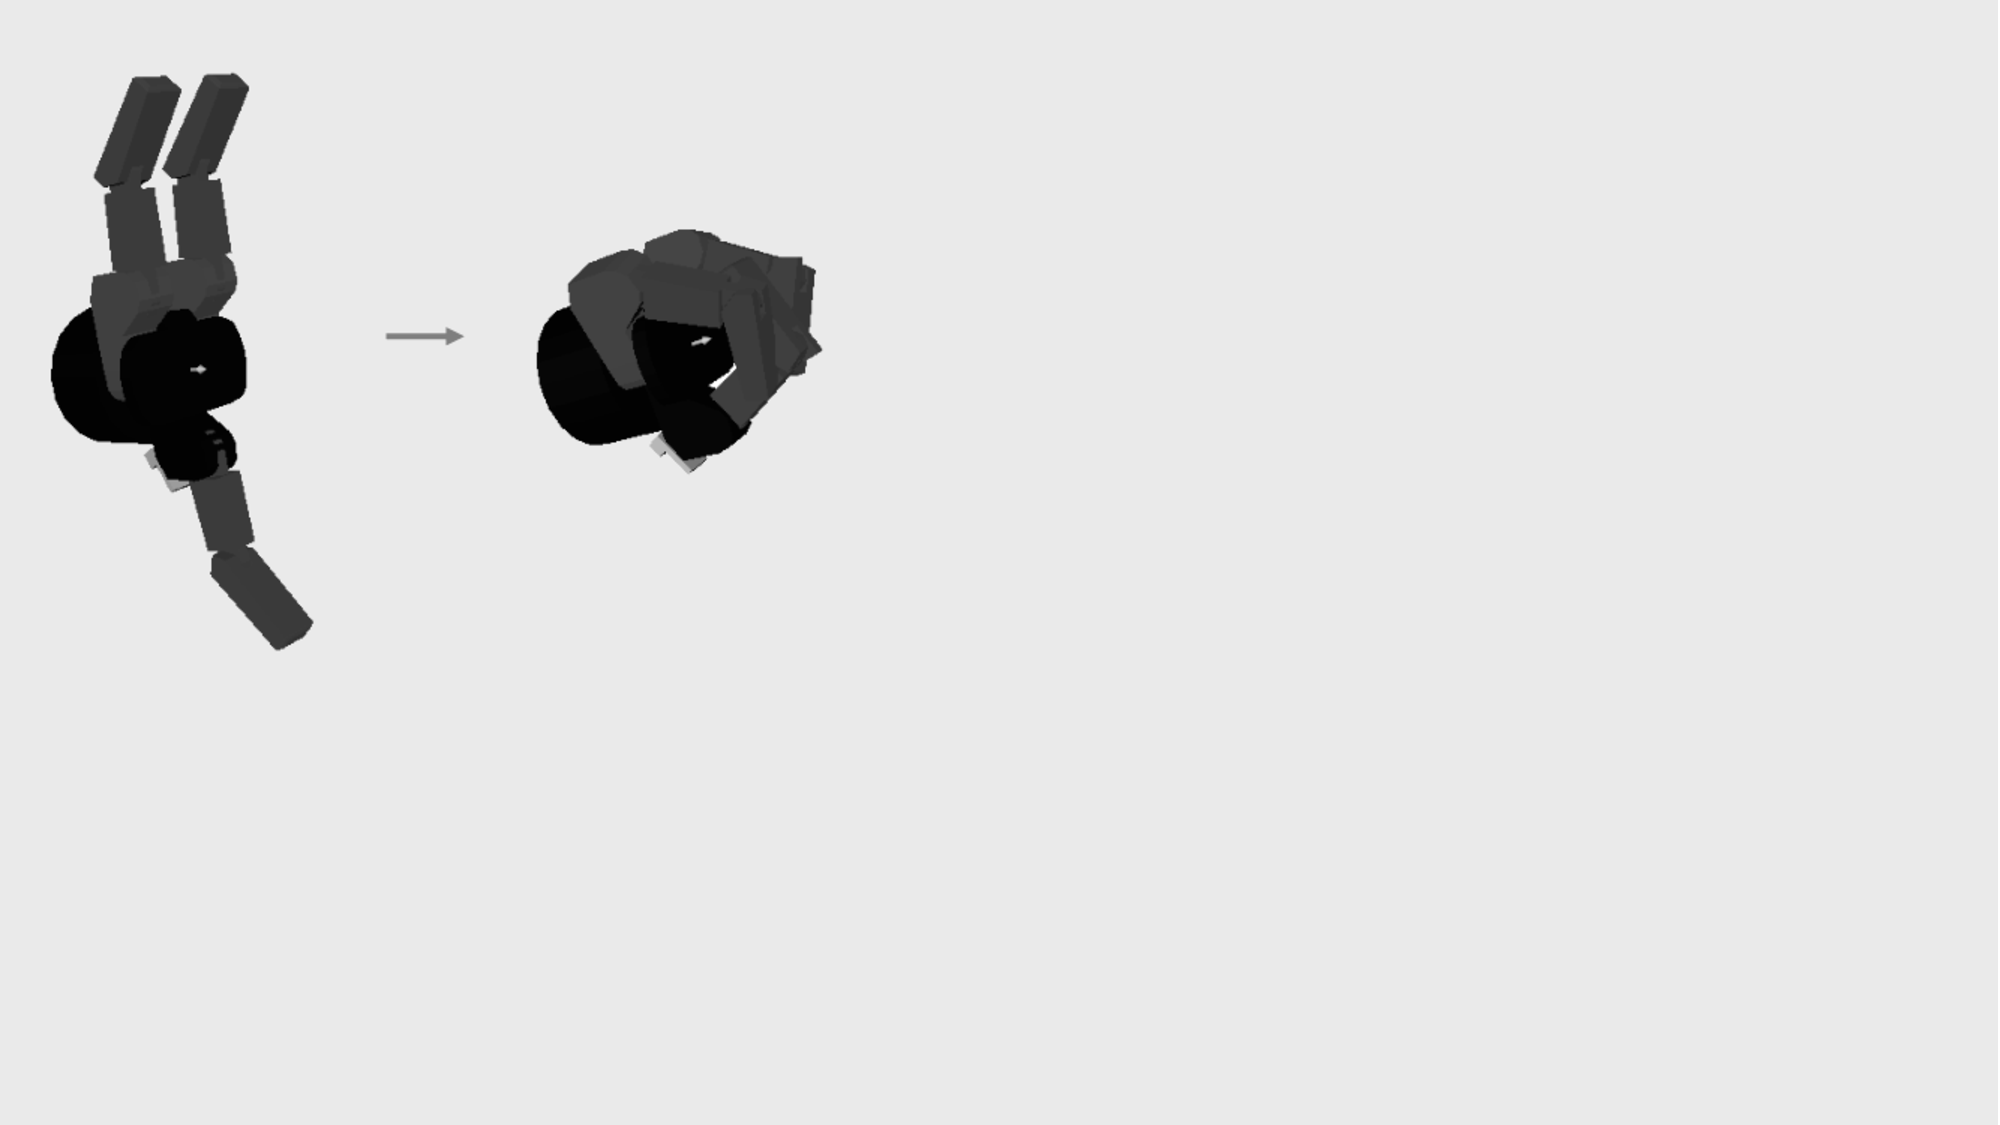
\includegraphics[trim={0.75cm 8cm 19cm 0.85cm},clip,width=1\linewidth,angle=0]{Apendices/Figuras/barret_eigengrasp_02.pdf}
				\caption{\textit{Eigengrasp} 02: fingers flexion.}
				\label{fig:barrett_eigengrasp02}
			\end{subfigure}
		\end{tcolorbox}
		\caption{The 4 \ac{DOF} Barrett gripper and its bidimensional \textit{eigengrasp} representation. }
		\label{fig:barrett_eigengrasps}
	}%end of resize box      
\end{figure}

The optimisation algorithm tries to minimize the distance from the \ac{ICP}, that constitute the \ac{ICR} (Figure~\ref{fig:icp_opt}), to the object surface by adjusting the discussed optimization variables $\mathbf{a}$ and $\mathbf{w}$. The \ac{ICR} is a contact region model (a predefined group of distributed \acp{ICP}) used to calculate the interaction of the algorithm, thus it is possible to create a feasible procedure. 

Therefore, the objective function to be minimised is described by Equation~\ref{eq:fob_grasp_complete}, where $N$ is the number of total contacts in \ac{ICR}, $\mathbf{\hat{n}}_{i}$ is the surface normal, $\mathbf{o}_{i}$ the distance between the \ac{ICP} and the object ($i \in N$). The scalar $\alpha$ is a range adjustment factor between the distance and the normalised dot product of the second sum part. It is important to note that the $\mathbf{o}_{i}$ and $\mathbf{\hat{n}}_{i}$ are updated according to 3D simulation interaction in the ``GraspIt!''~\cite{AndrewT2004}. %A detailed description of the algorithm procedure is presented in \cite{Ciocarlie2009}.    

\begin{equation}
Q=\sum_{i=1}^{N}\left(1-\delta_{i}\right)\hspace{0.5cm}\textnormal{with}\hspace{0.5cm}\delta_{i}=\frac{\left|\mathbf{o}_{i}\right|}{\alpha}+\left(1-\frac{\mathbf{\hat{n}}_{i} \cdot\mathbf{o}_{i}}{\left|\mathbf{o}_{i}\right|}\right)
\label{eq:fob_grasp_complete}
\end{equation}


\begin{figure}[h!] %because of cas-sc
\resizebox{1\textwidth}{!}{%
\begin{tcolorbox}
% \centerline{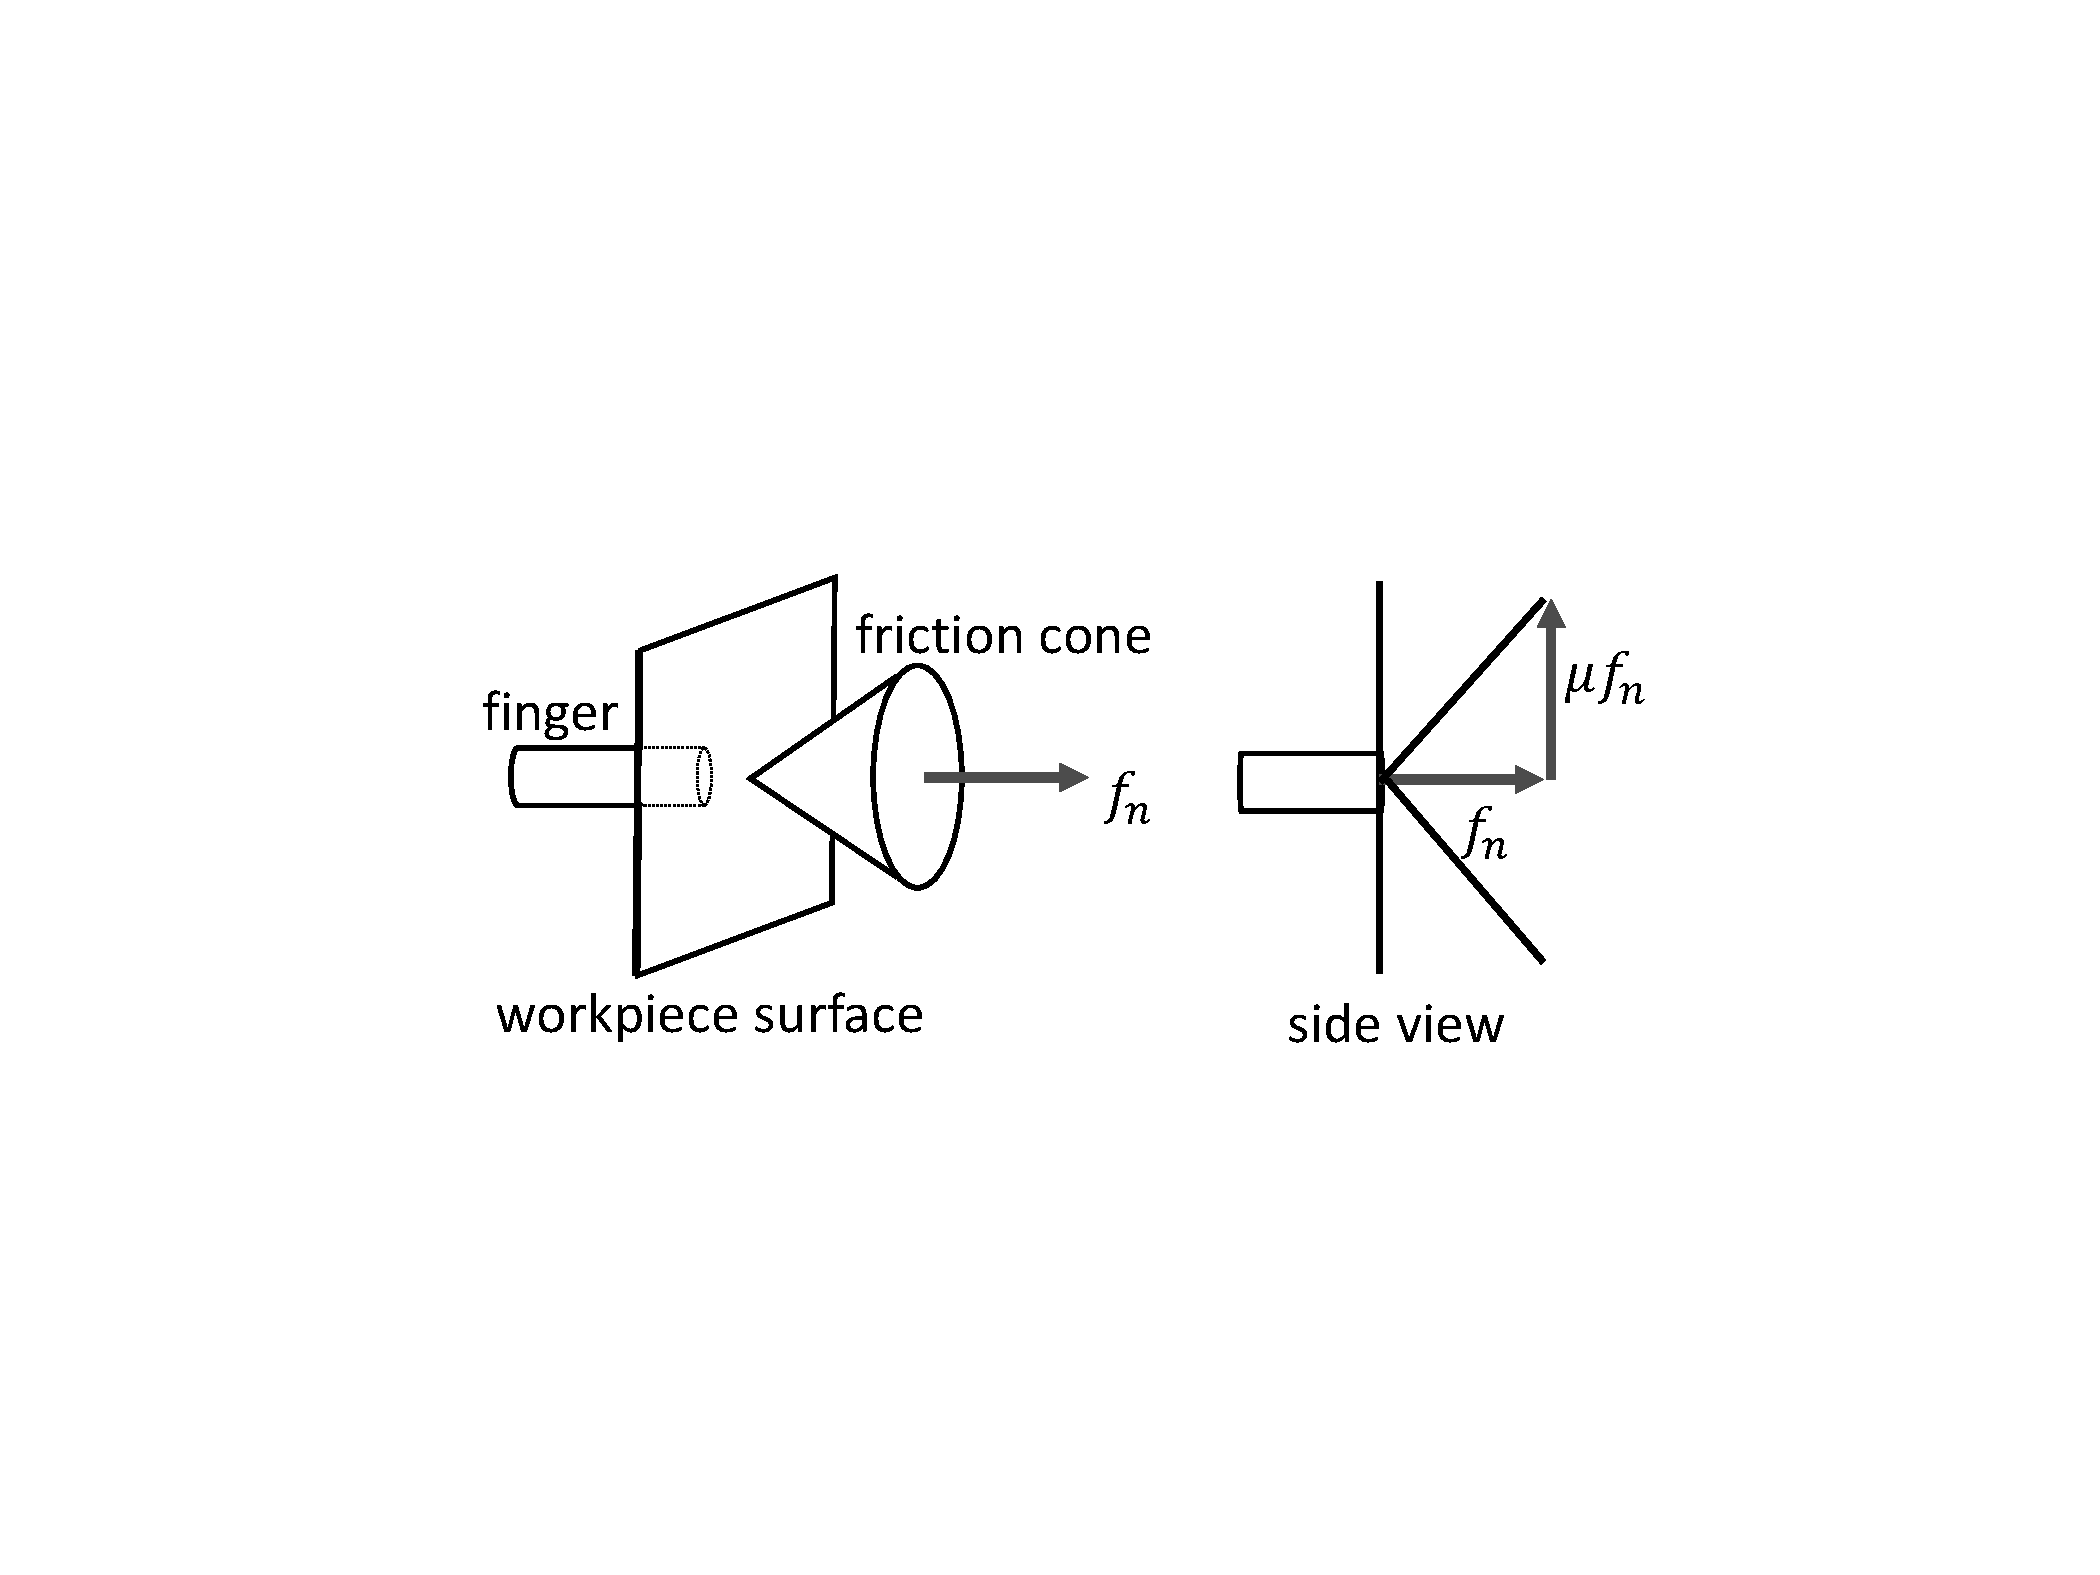
\includegraphics[trim={7cm 8cm 7cm 9cm},clip,width=1\linewidth,angle=0]{Cap2/Figuras/friction_contact.pdf}}
\centerline{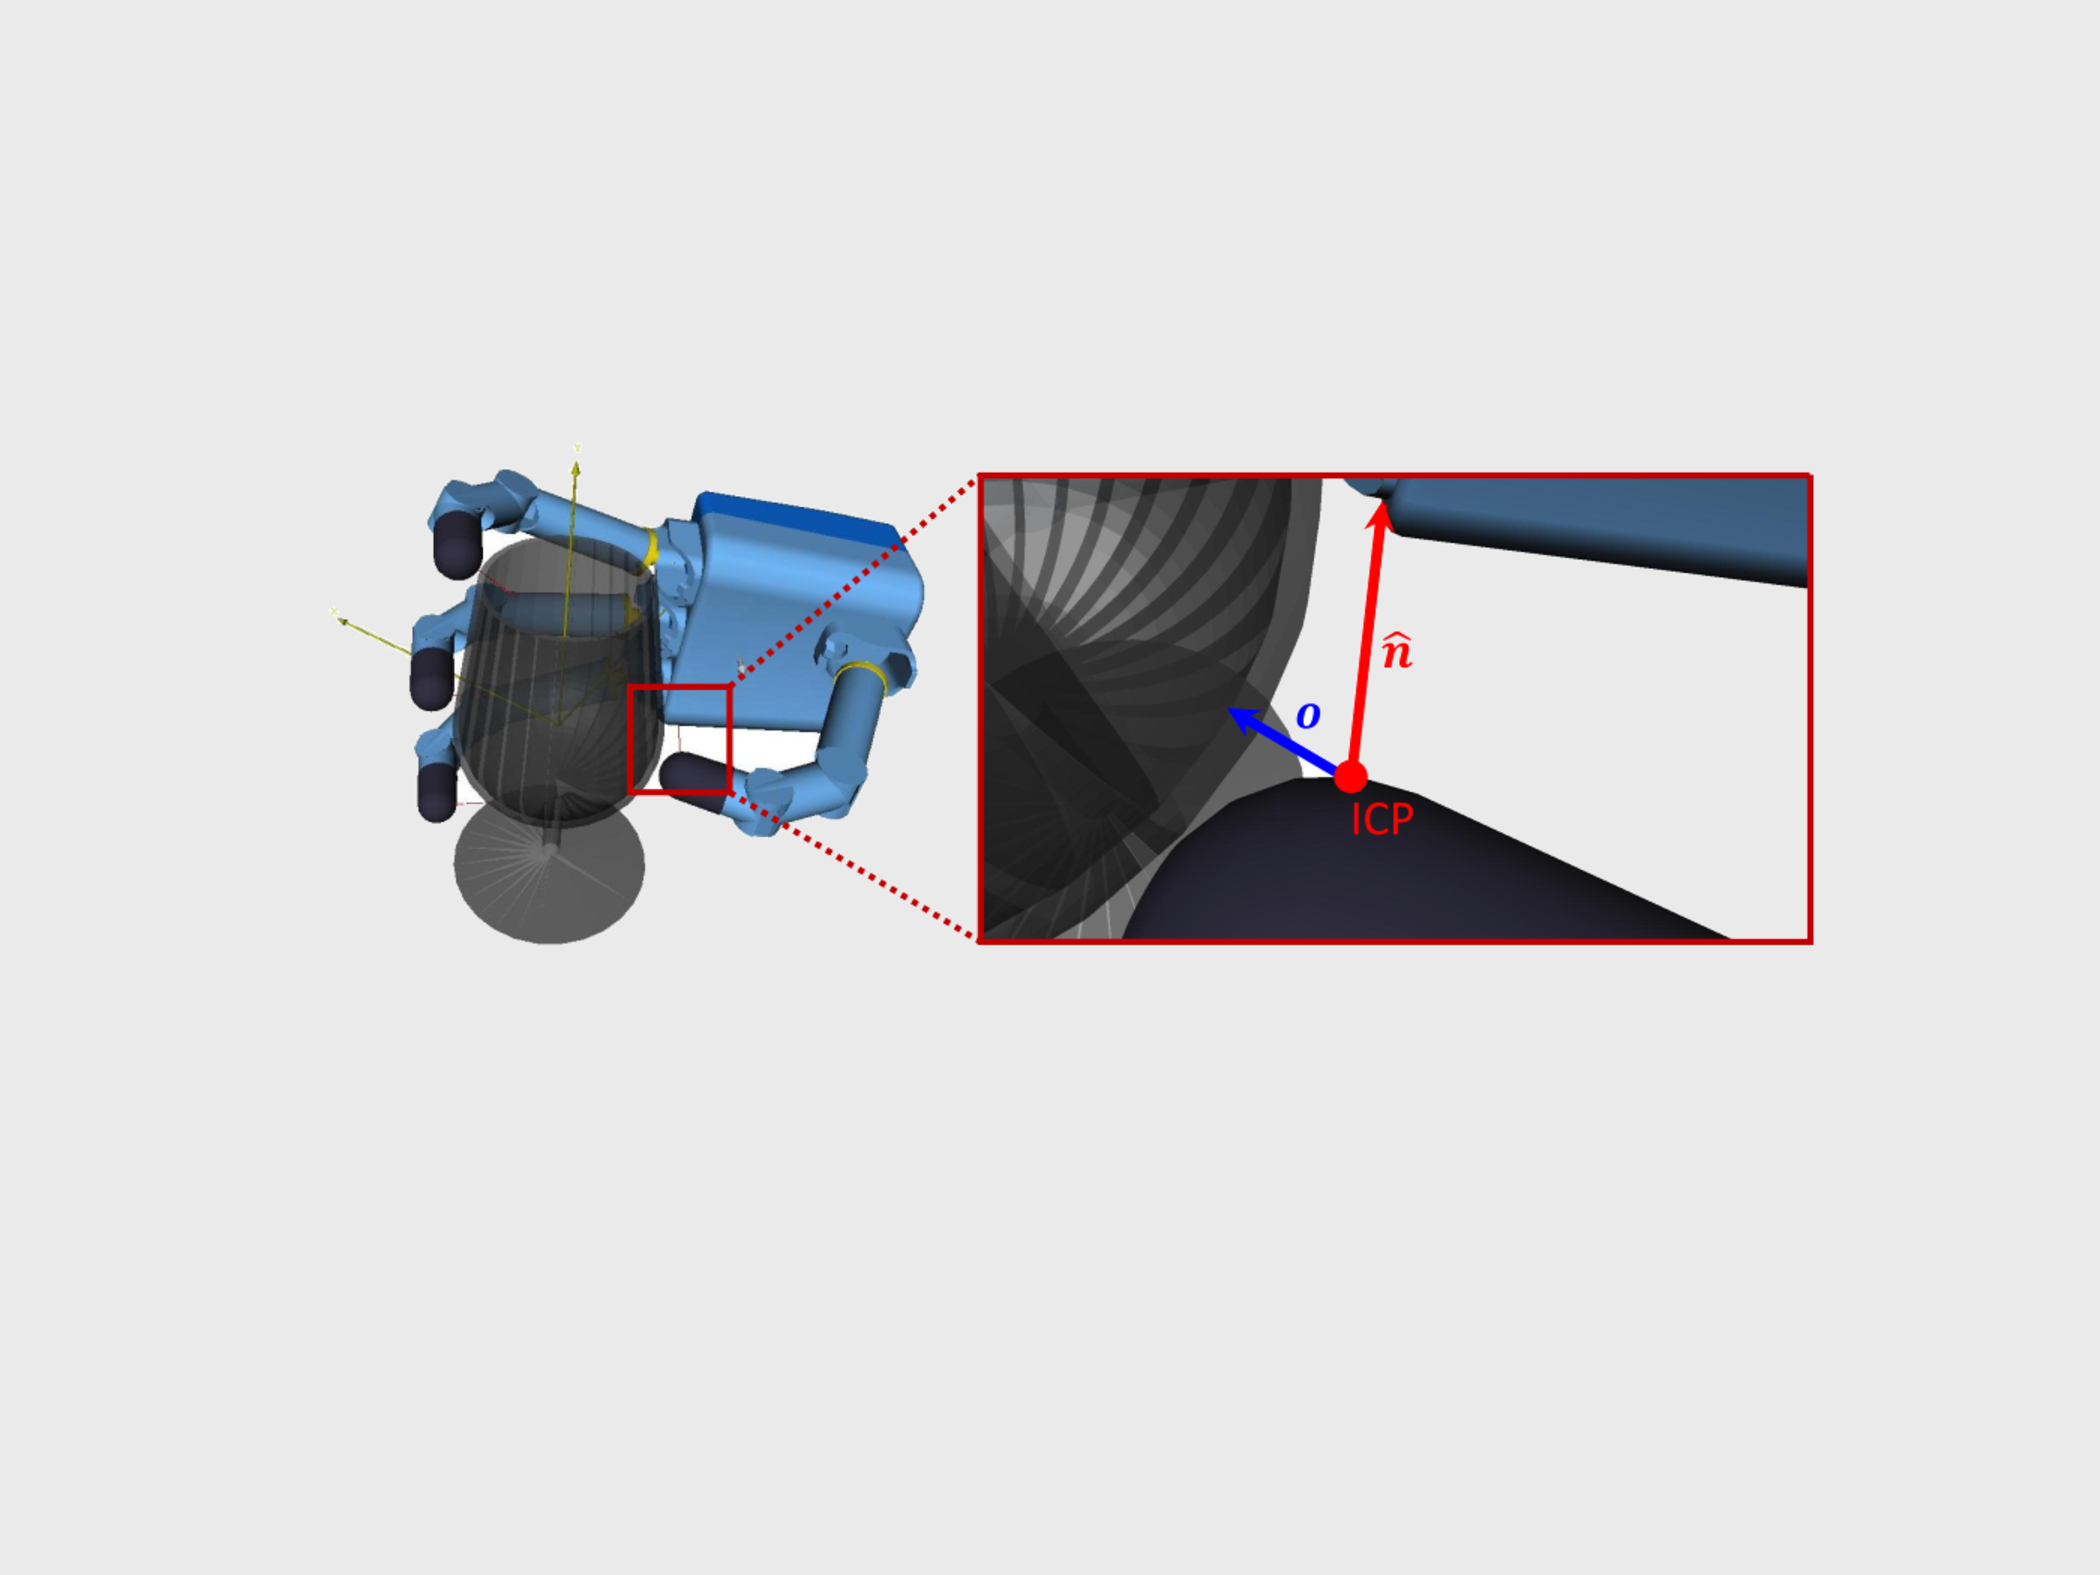
\includegraphics[trim={6.5cm 10cm 4cm 8cm},clip,width=1\linewidth,angle=0]{Apendices/Figuras/ICPreduction_gray_bg.pdf}}
\end{tcolorbox}
\caption{Grasping optimisation process elucidation.}
\label{fig:icp_opt}
}
\end{figure}


The algorithm proposed by~\cite{Ciocarlie2009}, and used in this proposal, is replicated in Algorithm~\ref{alg:snn_grasp}. As already mentioned, the variables that define the states are $\mathbf{a}$, related to the \textit{eigengrasp}, and $\mathbf{w}$, related to the wrist pose. The ``\textit{ObjFunc}'' is described by Equation~\ref{eq:fob_grasp_complete}. The ``\textit{Ngbr}'' is the calculus of the state variables neighbour values using the Equation~\ref{eq:neighbors} and, ``\textit{Probability}'' is the function to perform the jump probability to a new state according to Equation~\ref{eq:very_fast_snn_prob}. Since this step of the algorithm is based on ``GraspIt!''} the ``ForwardKinematics'' and collision check are parts of this tool.

 \begin{algorithm}[h!]
 	\centering
	\resizebox{0.85\textwidth}{!}{%
	\begin{tcolorbox}
		\ForAll {variables of CurrentState} 
		{CurrentState.variable = RandomValue()}
		QCurrent = ObjFunc(CurrentState)\;
		Steps = 0\;
		QSaved = 0\;
		\While{Steps $\neq$ MaxSteps}{
			\tcp{Generate a new state as a neighbour of current state}
			\Repeat{legalState == true}
			{
				\ForAll{variables of NewState}{
					\tcp{SANN neighbour generation function}
					NewState.variable = Ngbr(CurrentState.variable)\;
				}
				Apply ForwardKinematics(NewState)\;
				\If{collisions detected \textnormal{\textbf{or}} joint limits exceeded} {
					legalState = false\;
				} \Else{
					legalState = true
				}
				
			} 
			QNew = ObjFunc(NewState)\;
			\If{QNew $>$ QSaved}
			{
				Insert NewState in SavedStatesList\;
				QSaved = lowest ObjFunc value in SavedStateList\;
			}
			\tcp{SANN probability of "jumping" to new state}
			PJump = Probability(QCurrent, QNew)\;
			\If{PJump $>$ 0.5}{
				CurrentState = NewState\;
				QCurrent = QNew\;
			}
			Steps = Steps + 1\;
		}	
		 \end{tcolorbox}
		\caption{\ac{SANN} applied to grasping proposed by \cite{Ciocarlie2009}.}
		\label{alg:snn_grasp}
		}
\end{algorithm}